\documentclass[aspectratio=169,10pt]{beamer}

\usetheme{Madrid}
\usepackage[T1]{fontenc}
\usepackage{lmodern}
\usepackage{graphicx}
\usepackage{booktabs}
\usepackage{array}
\usepackage{amsmath}
\usepackage{tikz}
\usetikzlibrary{positioning,arrows.meta,calc,shapes.geometric,fit,backgrounds}

\definecolor{navy}{RGB}{24,45,86}
\definecolor{accent}{RGB}{176,54,40}
\definecolor{soft}{RGB}{236,240,247}
\setbeamercolor{structure}{fg=navy}
\setbeamercolor{palette primary}{bg=navy,fg=white}
\setbeamercolor{palette secondary}{bg=navy!85!black,fg=white}
\setbeamercolor{palette tertiary}{bg=navy!70!black,fg=white}
\setbeamercolor{title}{bg=navy,fg=white}
\setbeamercolor{frametitle}{bg=soft,fg=navy}
\setbeamercolor{block title}{bg=navy,fg=white}
\setbeamercolor{block body}{bg=soft}
\setbeamertemplate{navigation symbols}{}
\setbeamertemplate{itemize items}[circle]
\setbeamerfont{frametitle}{size=\large,series=\bfseries}
\setbeamerfont{block title}{size=\small,series=\bfseries}
\newcommand{\expsize}{\scriptsize}

\newcommand{\hl}[1]{\textcolor{accent}{\textbf{#1}}}
\newcommand{\takeaway}[1]{\par\vspace{2pt}{\small\textcolor{navy}{\textbf{Takeaway:}} #1}}

% card for one module: title, why, what, result
\newcommand{\modcard}[4]{%
  \begin{block}{#1}\footnotesize
    \textcolor{navy}{\textbf{Why:}} #2\\[1pt]
    \textcolor{navy}{\textbf{What:}} #3\\[1pt]
    \textcolor{navy}{\textbf{Result:}} #4
  \end{block}}
% card for one experiment: title, why, result, takeaway
\newcommand{\expcard}[4]{%
  \begin{block}{#1}\expsize
    \textcolor{navy}{\textbf{Why:}} #2\\[1pt]
    \textcolor{navy}{\textbf{Result:}} #3\\[1pt]
    \textcolor{navy}{\textbf{Takeaway:}} #4
  \end{block}}
% one example item: label, sub-question, answer, reason
\newcommand{\excard}[4]{%
  \begin{block}{#1}\scriptsize
    \textcolor{navy}{\textbf{Sub-question:}} #2\\[3pt]
    \textcolor{navy}{\textbf{Answer:}} \emph{#3}\\[3pt]
    \textcolor{navy}{\textbf{Why this label:}} #4
  \end{block}}

\title[Knowledge over Structure]{Knowledge over Structure}
\subtitle{A Controlled Study of Response Clarity Classification in Political Interviews\\[2pt]
  \small SemEval-2026 Task 6 (CLARITY)}
\author[Team Nier\_ANLP]{Vidvathama R \and Siddarth Gottumukkula \and Sanjana Reddy Vonteri \and Shashikanta Sahoo\texorpdfstring{\\[2pt]\small Team Nier\_ANLP}{}}
\institute[IIIT Hyderabad]{International Institute of Information Technology, Hyderabad}
\date[October 2026]{Advanced NLP \quad\textbullet\quad October 2026}

\begin{document}

% 1
\begin{frame}
  \titlepage
\end{frame}

% 2
\begin{frame}{What are we classifying? Three real dev items}
  \begin{columns}[T]
    \begin{column}{0.32\textwidth}
      \excard{Clear Reply \quad$\rightarrow$\quad Explicit}
        {``Do you stand by your figure, 30,000?''}
        {``You know, I stand by the figure. A lot of innocent people have lost their life---600,000, or whatever they guessed at, is just---it's not credible. \ldots''}
        {he states the requested position outright.}
    \end{column}
    \begin{column}{0.32\textwidth}
      \excard{Ambivalent \quad$\rightarrow$\quad Dodging}
        {``Do you see a risk of triggering a wider war?''}
        {``I thought you were going to ask me about the pig.''}
        {he ignores the question and changes the subject.}
    \end{column}
    \begin{column}{0.32\textwidth}
      \excard{Clear Non-Reply \quad$\rightarrow$\quad Declining}
        {``Is it a fair assumption that the CIA operatives are in Pakistan, cooperating with the Pakistanis, and that they're sharing everything with you and vice versa?''}
        {``John, what's fair is, I'm not---what you must assume is that I'm not going to talk about ongoing intelligence matters. \ldots''}
        {he openly refuses to give the information.}
    \end{column}
  \end{columns}
  \vspace{6pt}
  \begin{itemize}\small
    \item All three annotators agree on each of these. The ``pig'' answer is attached to all three sub-questions of its turn, so the model must work out \emph{which part} of an answer responds to \emph{which} sub-question.
    \item We predict the 9-way evasion type (Subtask 2). The 3-way clarity level (Subtask 1) follows from it.
  \end{itemize}
\end{frame}

% 3
\begin{frame}{The task: how clearly does a politician answer?}
  \begin{columns}[T]
    \begin{column}{0.55\textwidth}
      Each item pairs one \textbf{sub-question} from a journalist's turn, the \textbf{full question}, and the
      politician's \textbf{answer}. We predict the 9-way label and map it to the 3-way one.
      \vspace{6pt}

      {\small
      \begin{tabular}{@{}>{\raggedright\arraybackslash}p{2.3cm}>{\raggedright\arraybackslash}p{3.7cm}r@{}}
        \toprule
        Subtask 1 & Subtask 2 & train \\
        \midrule
        Clear Reply & Explicit & 30.5\% \\
        Ambivalent & Implicit, Dodging, General, Deflection, Partial/half-answer & 59.2\% \\
        Clear Non-Reply & Declining to answer, Claims ignorance, Clarification & 10.3\% \\
        \bottomrule
      \end{tabular}}
    \end{column}
    \begin{column}{0.42\textwidth}
      \begin{block}{Data and metric}
        \small
        \begin{itemize}
          \item Train 3,448 rows. Dev 308 items (3 annotators). Test 237 (2 annotators, labels unreleased)
          \item Macro-F1 over 9 classes. A prediction counts if \emph{any} annotator gave it
          \item All numbers are on dev
        \end{itemize}
      \end{block}
      \begin{block}{Why it is hard}
        \small
        \begin{itemize}
          \item 69\% of rows share their answer with another sub-question
          \item Humans disagree: one annotator vs.\ the other two scores \hl{0.684}
        \end{itemize}
      \end{block}
    \end{column}
  \end{columns}
\end{frame}

% 4
\begin{frame}{Baselines: what the other teams did}
  \centering\scriptsize
  \renewcommand{\arraystretch}{0.95}\setlength{\tabcolsep}{5pt}
  \begin{tabular}{@{}c c l l c c@{}}
    \toprule
    \multicolumn{2}{c}{\textbf{Rank}} & \textbf{Team} & \textbf{Approach} & \textbf{S1} & \textbf{S2} \\
    S2 & S1 & & & \multicolumn{2}{c}{test macro-F1} \\
    \midrule
    1  & 1  & \hl{TeleAI}                & DeepSeek-V3, 3 confidence-routed CoT stages, predicts S2 then maps to S1 & \hl{0.89} & \hl{0.68} \\
    2  & 7  & ChulaNLP (moswisarut)      & fine-tuned DeBERTa-large top-5 labels $\rightarrow$ few-shot Kimi-K2 & 0.82 & 0.61 \\
    3  & 9  & CLaC                       & prompted LLMs, ahead of their fine-tuned encoders & 0.80 & 0.59 \\
    4  & 4  & Rasende Rakete             & \textcolor{gray}{not described} & 0.83 & 0.59 \\
    5  & 6  & YNU-HPCC                   & \textcolor{gray}{not described} & 0.83 & 0.59 \\
    \midrule
    7  & 3  & CSE-UOI                    & Grok 4.1 + Gemini 3 Flash, weighted vote with difficulty gating & 0.85 & 0.58 \\
    8  & 13 & ttda704                    & structured chain-of-thought prompting & 0.79 & 0.56 \\
    9  & 5  & Evaluators                 & LoRA-tuned open LLMs & 0.83 & 0.54 \\
    12 & 18 & PFW (taleef)               & 50 DeBERTa models averaged (5 folds $\times$ 10 seeds) & 0.76 & 0.50 \\
    17 & 8  & tahamunawar                & encoder with NLI reframing, multi-task, GNN, MIL & 0.81 & 0.45 \\
    -- & 2  & AsymVerify                 & GPT-5.2, three confidence-gated verification passes & 0.85 & -- \\
    -- & 14 & SilkPeak                   & one DeBERTa-v3-large with joint clarity and evasion heads & 0.76 & -- \\
    \midrule
    \multicolumn{3}{@{}l}{\textit{Organiser baseline}} & fine-tuned Llama-70B (Thomas et al., 2024) & 0.82 & 0.57 \\
    \bottomrule
  \end{tabular}\par\vspace{4pt}
  \begin{itemize}\footnotesize
    \item 41 teams in S1, 33 in S2. Only 7 beat the S2 baseline, and the S2 median is about 0.52.
    \item The top systems are LLM pipelines that use the taxonomy. Encoders level off near \hl{0.50 on S2}.
  \end{itemize}
  {\tiny Test scores (237 items) from the task overview paper, Table 3. Approaches from the overview and the teams' system papers. Our numbers are on dev, so they are not directly comparable.}
\end{frame}

% 5
\begin{frame}{How the work progressed}
  \centering
  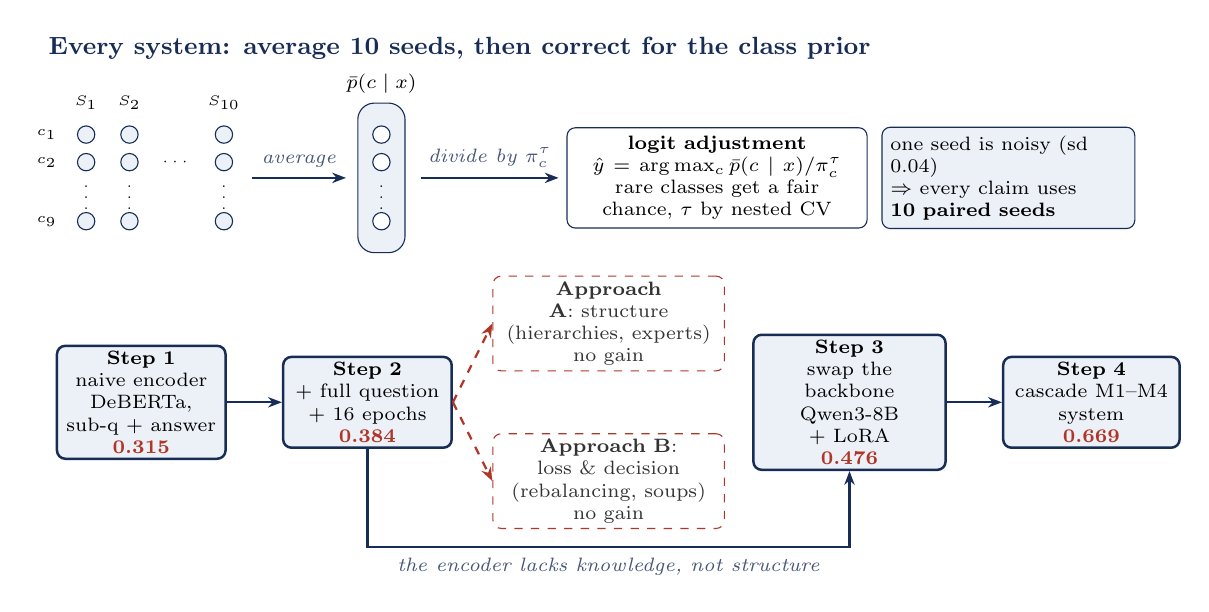
\begin{tikzpicture}[
      font=\scriptsize,
      dot/.style={circle, draw=navy, fill=soft, minimum size=2.2mm, inner sep=0pt},
      phase/.style={draw=navy, rounded corners=3pt, align=center, fill=white, text width=20mm, minimum height=11mm, inner sep=2pt},
      good/.style={phase, fill=soft, line width=0.9pt},
      bad/.style={phase, dashed, draw=accent, text=black!80, text width=28mm, minimum height=8mm},
      arr/.style={-{Stealth[length=5pt]}, navy, thick},
      lab/.style={font=\scriptsize\itshape, text=navy!80}]
    % top: how every system decides (seeds -> mean -> prior correction)
    \node[anchor=west, font=\small\bfseries, text=navy] at (-0.6,2.75) {Every system: average 10 seeds, then correct for the class prior};
    \foreach \s/\x in {1/0, 2/0.55, 10/1.75} {
      \node[font=\tiny] at (\x,2.05) {$S_{\s}$};
      \foreach \y in {1.65,1.3,0.55} { \node[dot] at (\x,\y) {}; }
      \node[font=\tiny] at (\x,0.95) {$\vdots$};
    }
    \node[font=\tiny] at (1.15,1.3) {$\cdots$};
    \node[font=\tiny, anchor=east] at (-0.25,1.65) {$c_1$};
    \node[font=\tiny, anchor=east] at (-0.25,1.3) {$c_2$};
    \node[font=\tiny, anchor=east] at (-0.25,0.55) {$c_9$};
    \draw[arr] (2.1,1.1) -- node[lab, above] {average} (3.3,1.1);
    \node[draw=navy, rounded corners=6pt, minimum width=6mm, minimum height=19mm, fill=soft] (pbar) at (3.75,1.1) {};
    \foreach \y in {1.65,1.3,0.55} { \node[dot, fill=white] at (3.75,\y) {}; }
    \node[font=\tiny] at (3.75,0.95) {$\vdots$};
    \node[font=\scriptsize] at (3.75,2.3) {$\bar p(c\mid x)$};
    \draw[arr] (4.25,1.1) -- node[lab, above] {divide by $\pi_c^{\tau}$} (6.0,1.1);
    \node[draw=navy, rounded corners=3pt, align=center, fill=white, text width=36mm, inner sep=3pt, anchor=west] at (6.1,1.1)
      {\textbf{logit adjustment}\\$\hat y=\arg\max_c \bar p(c\mid x)/\pi_c^{\tau}$\\rare classes get a fair chance, $\tau$ by nested CV};
    \node[draw=navy, rounded corners=3pt, align=left, fill=soft, text width=30mm, inner sep=3pt, anchor=west] at (10.1,1.1)
      {one seed is noisy (sd 0.04)\\$\Rightarrow$ every claim uses\\\textbf{10 paired seeds}};
    % bottom: the phases
    \node[good] (s1) at (0.7,-1.75) {\textbf{Step 1}\\naive encoder\\DeBERTa, sub-q + answer\\\hl{0.315}};
    \node[good, right=7mm of s1] (s2) {\textbf{Step 2}\\+ full question\\+ 16 epochs\\\hl{0.384}};
    \node[bad, above right=-2mm and 5mm of s2] (a) {\textbf{Approach A}: structure\\(hierarchies, experts)\\no gain};
    \node[bad, below right=-2mm and 5mm of s2] (b) {\textbf{Approach B}: loss \& decision\\(rebalancing, soups)\\no gain};
    \node[good, right=38mm of s2, text width=23mm] (s3) {\textbf{Step 3}\\swap the backbone\\Qwen3-8B + LoRA\\\hl{0.476}};
    \node[good, right=7mm of s3, text width=21mm] (s4) {\textbf{Step 4}\\cascade M1--M4\\system\\\hl{0.669}};
    \draw[arr] (s1) -- (s2);
    \draw[arr, accent, dashed] (s2.east) -- (a.west);
    \draw[arr, accent, dashed] (s2.east) -- (b.west);
    \draw[arr] (s2.south) -- ++(0,-1.25) -| node[lab, pos=0.25, below] {the encoder lacks knowledge, not structure} (s3.south);
    \draw[arr] (s3) -- (s4);
  \end{tikzpicture}
  \vspace{2pt}

  {\footnotesize Numbers are dev Subtask 2 macro-F1 for one model (mean of 10 seeds), except Step 4, which is the full system.}
\end{frame}

% 6
\begin{frame}{The classification pipeline shared by both backbones}
  \centering
  \resizebox{\textwidth}{!}{% Figure 1: the classification pipeline (TikZ, monochrome). Input by \FigureArch in figs.tex.
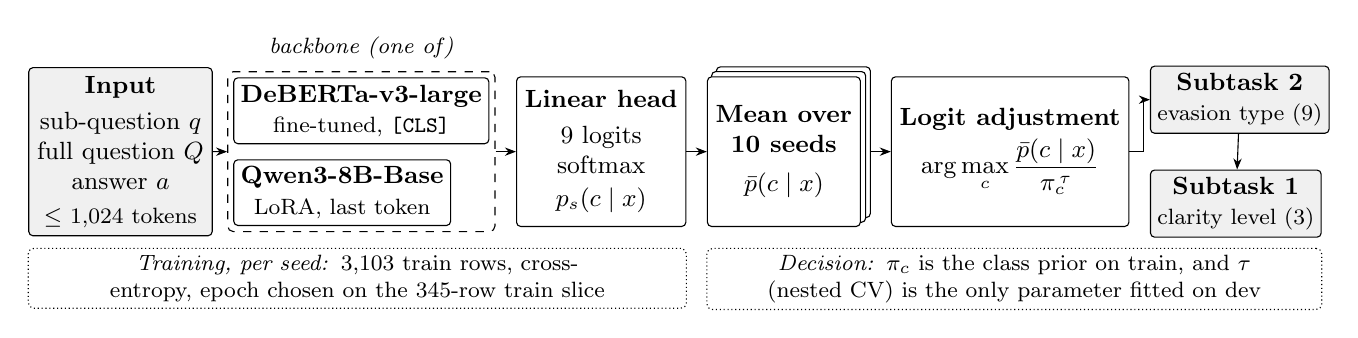
\begin{tikzpicture}[
  font=\small,
  node distance=2.6mm,
  box/.style={draw, rounded corners=1.5pt, align=center, inner xsep=3pt, inner ysep=3pt, minimum height=#1},
  box/.default=19mm,
  sub/.style={draw, rounded corners=1.5pt, align=center, inner sep=2.5pt, minimum width=#1},
  sub/.default=25mm,
  arr/.style={-{Stealth[length=4pt]}, thin},
  note/.style={font=\footnotesize\itshape, align=center},
  band/.style={draw, densely dotted, rounded corners=2pt, inner sep=2.5pt, align=center, font=\footnotesize},
]
% Input
\node[box, fill=black!6] (in) {%
  \textbf{Input}\\[2pt]
  sub-question $q$\\
  full question $Q$\\
  answer $a$\\[1pt]
  {\footnotesize $\le$ 1{,}024 tokens}};

% Backbone: one of two
\node[sub, right=of in, yshift=5.2mm] (deb) {\textbf{DeBERTa-v3-large}\\{\footnotesize fine-tuned, \texttt{[CLS]}}};
\node[sub, right=of in, yshift=-5.2mm] (qwen) {\textbf{Qwen3-8B-Base}\\{\footnotesize LoRA, last token}};
\node[draw, dashed, rounded corners=2pt, inner sep=2pt, fit=(deb)(qwen)] (bb) {};
\node[note, above=0.3mm of bb] {backbone (one of)};

% Head
\node[box, right=of bb] (head) {\textbf{Linear head}\\[2pt] 9 logits\\ softmax\\[1pt] $p_s(c \mid x)$};

% Seed ensemble: stacked outlines stand for the ten trained seeds
\node[box, right=of head, fill=white] (ens) {\textbf{Mean over}\\\textbf{10 seeds}\\[3pt] $\bar p(c \mid x)$};
\begin{scope}[on background layer]
  \draw[rounded corners=1.5pt, fill=white] ($(ens.south west)+(1.2mm,1.2mm)$) rectangle ($(ens.north east)+(1.2mm,1.2mm)$);
  \draw[rounded corners=1.5pt, fill=white] ($(ens.south west)+(0.6mm,0.6mm)$) rectangle ($(ens.north east)+(0.6mm,0.6mm)$);
\end{scope}

% Logit adjustment
\node[box, right=of ens, xshift=1.2mm] (la) {\textbf{Logit adjustment}\\[2pt]
  $\arg\max\limits_c \dfrac{\bar p(c \mid x)}{\pi_c^{\,\tau}}$};

% Outputs
\node[sub=20mm, fill=black!6, right=of la, yshift=6.6mm] (s2) {\textbf{Subtask 2}\\{\footnotesize evasion type (9)}};
\node[sub=20mm, fill=black!6, right=of la, yshift=-6.6mm] (s1) {\textbf{Subtask 1}\\{\footnotesize clarity level (3)}};

% Arrows
\draw[arr] (in) -- (bb);
\draw[arr] (bb) -- (head);
\draw[arr] (head) -- (ens);
\draw[arr] ($(ens.east)+(1.2mm,0)$) -- (la);
\draw[arr] (la.east) -- ++(1.8mm,0) |- (s2.west);
\draw[arr] (s2) -- (s1);

% Training and decision notes
\path let \p1=(in.west), \p2=(head.east), \p3=(bb.south) in
  node[band, anchor=north, text width=\x2-\x1-5pt] at ({(\x1+\x2)/2}, \y3-2mm) (train) {%
  \textit{Training, per seed:} 3{,}103 train rows, cross-entropy, epoch chosen on the 345-row train slice};
\path let \p1=(ens.west), \p2=(s1.east), \p3=(train.north) in
  node[band, anchor=north, text width=\x2-\x1-5pt] at ({(\x1+\x2)/2}, \y3) (dec) {%
  \textit{Decision:} $\pi_c$ is the class prior on train, and $\tau$ (nested CV) is the only parameter fitted on dev};
\end{tikzpicture}
}
  \vspace{6pt}
  \begin{itemize}\small
    \item \textbf{Backbone (one of two):} DeBERTa-v3-large, fully fine-tuned, reads the \texttt{[CLS]} state. Qwen3-8B-Base with LoRA reads the last token. Both see the sub-question $q$, the full question $Q$ and the answer $a$ ($\le$ 1,024 tokens).
    \item \textbf{Head:} a new linear layer gives 9 logits and a softmax $p_s(c\mid x)$ over the evasion types for each seed $s$.
    \item \textbf{System:} average the 10 seeds into $\bar p(c\mid x)$, then divide by the train class prior $\pi_c$ raised to $\tau$.
    \item \textbf{Output:} the Subtask 2 label (9 types) fixes the Subtask 1 clarity level (3) through the taxonomy.
  \end{itemize}
\end{frame}

% 7
\begin{frame}{Phase 1: a carefully controlled encoder (DeBERTa-v3-large)}
  \centering
  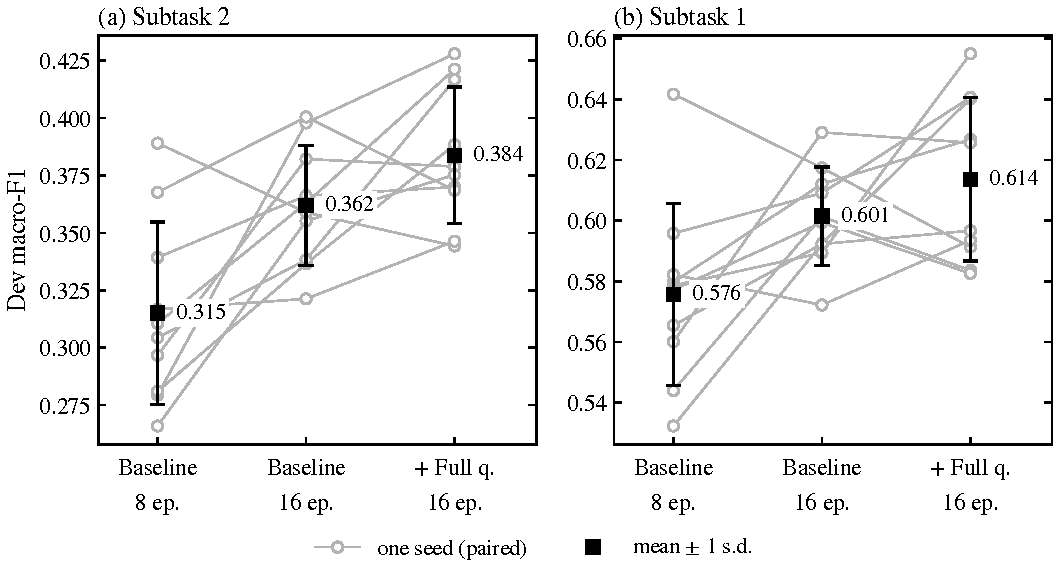
\includegraphics[height=0.56\textheight]{figures/deberta_seeds.pdf}
  \vspace{2pt}
  \begin{itemize}\small
    \item[] \textcolor{navy}{\textbf{Why:}} our first encoder trailed ChulaNLP's (0.46), and 69\% of rows share an answer, so the model needs the full question.
    \item[] \textcolor{navy}{\textbf{Result:}} 16 epochs + full question: \hl{0.315 $\rightarrow$ 0.384} per model (+0.069, 9/10 seeds up). System 0.405 S2 / 0.648 S1.
    \item[] \textcolor{navy}{\textbf{Takeaway:}} undertraining hid the gain (at 8 epochs, 0.282 vs 0.337, loss still 1.3--1.5), so we report fit next to every score.
  \end{itemize}
\end{frame}

% 8
\begin{frame}{Encoder experiments (1/3): the decision rule and the re-ranker}
  \begin{columns}[c]
    \begin{column}{0.46\textwidth}
      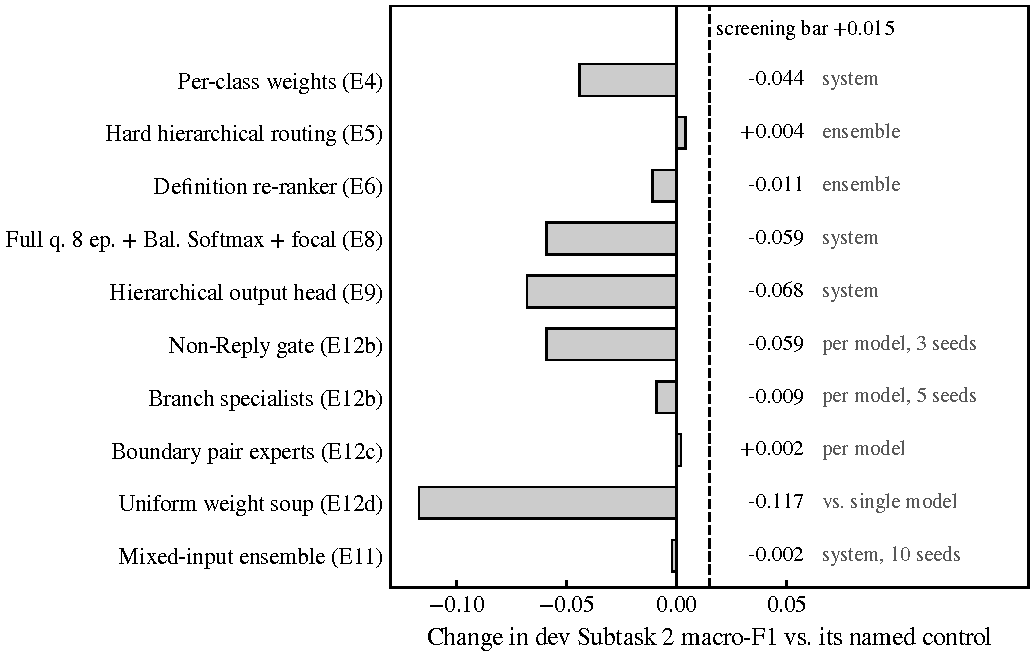
\includegraphics[width=\linewidth]{figures/negative_results.pdf}
    \end{column}
    \begin{column}{0.52\textwidth}
      \expcard{E4 \quad Per-class decision weights}
        {argmax ignores macro-F1's equal class weights and dev's different label mix.}
        {logit adjustment 0.365 $\rightarrow$ \hl{0.438}. Nine weights reach only 0.394 (in-fold gap +0.098).}
        {one scalar $\tau$ beats nine weights on 308 items. Every system uses it.}
      \expcard{E5 \quad Hard routing through the clarity level}
        {the organisers report that using the taxonomy hierarchy helps.}
        {0.369 vs 0.365 for the flat model (5-seed ensemble).}
        {no reliable effect. The model's own top 3 (89.6\% hit) beats the taxonomy branch (81.2\%).}
      \expcard{E6 \quad Definition re-ranker over the top 3}
        {gold is in the top 3 for 89.6\% of items. A perfect chooser would score 0.745.}
        {0.354 vs 0.365. It fixes 25 errors but breaks 37 correct answers.}
        {label meaning needs knowledge that 3,400 examples cannot give. An LLM belongs here.}
    \end{column}
  \end{columns}
\end{frame}

% 9
\begin{frame}{Encoder experiments (2/3): losses, hierarchies and ensembles}
  \renewcommand{\expsize}{\small}
  \begin{columns}[T]
    \begin{column}{0.32\textwidth}
      \expcard{E8 \quad Balanced Softmax + focal loss}
        {rare classes were under-predicted, and Partial/half-answer never.}
        {system 0.379 vs 0.438. Explicit F1 fell by 0.36.}
        {the loss over-corrects towards rare classes. Logit adjustment does this job for free.}
    \end{column}
    \begin{column}{0.32\textwidth}
      \expcard{E9 \quad Factorised hierarchical head}
        {post-hoc routing failed, so we trained the hierarchy into the head instead.}
        {S2 0.370 vs 0.438 ($-$0.068). S1 +0.020, within noise.}
        {the flat softmax already scores all nine labels jointly.}
    \end{column}
    \begin{column}{0.32\textwidth}
      \expcard{E11 \quad Mixed-input ensemble}
        {an exploratory mix of full-question and base models scored 0.498 on dev.}
        {on fresh seeds 5--9: 0.403 vs 0.405 for full-question models alone.}
        {ideas found on dev need fresh-seed replication. We pre-register since.}
    \end{column}
  \end{columns}
  \vspace{8pt}
  \centering\small All changes are measured against a named control on paired seeds. A change must first pass a \hl{+0.015} 3-seed screen.
\end{frame}

% 10
\begin{frame}{Encoder experiments (3/3): soups, specialists and more data}
  \renewcommand{\expsize}{\small}
  \begin{columns}[T]
    \begin{column}{0.32\textwidth}
      \expcard{E12d \quad Model soups}
        {one model with part of the ensemble's gain, at no extra training cost.}
        {uniform soup of 10 models 0.267 vs 0.384 per model.}
        {seeds do not share a basin. Average the outputs, not the weights.}
    \end{column}
    \begin{column}{0.32\textwidth}
      \expcard{E12b/c \quad Specialists and pair experts}
        {Non-Reply recall was 0.57, and three confused pairs held most errors.}
        {gate $-$0.059. Specialists +0.018 at 3 seeds, $-$0.009 at 5. Pair experts +0.002.}
        {extra encoders re-decide what the flat model decides from the same input.}
    \end{column}
    \begin{column}{0.32\textwidth}
      \expcard{E12a \quad Training on all of train}
        {picking the epoch on the slice bought little, and all data adds 11\% rows.}
        {+0.029 S2 per model (4/5 seeds up), but S1 $-$0.017.}
        {the only variant that helped S2, but 5 seeds cannot rank it.}
    \end{column}
  \end{columns}
  \vspace{8pt}
  \centering\small Nothing trained on the same 3,448 rows moved the system. \hl{So we changed the backbone itself.}
\end{frame}

% 11
\begin{frame}{Where the encoder fails}
  \begin{columns}[c]
    \begin{column}{0.5\textwidth}
      \centering
      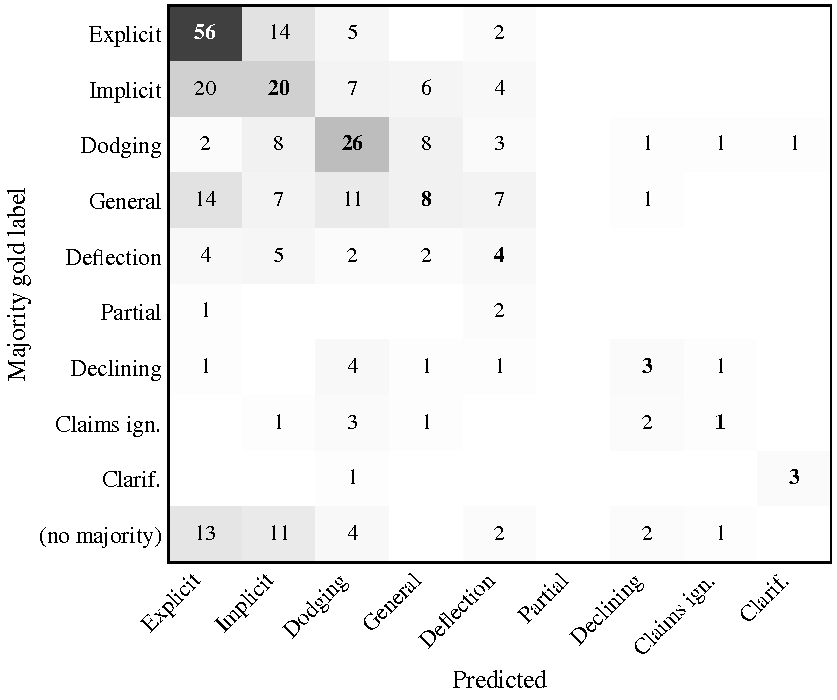
\includegraphics[width=\linewidth,height=0.78\textheight,keepaspectratio]{figures/confusion.pdf}
    \end{column}
    \begin{column}{0.46\textwidth}
      \footnotesize
      \begin{block}{How to read it}
        \footnotesize
        \begin{itemize}
          \item \textbf{Majority gold label}: the label that at least 2 of the 3 annotators chose. When all three differ (33 items), the item goes to the ``no majority'' row.
          \item Columns: the final DeBERTa 10-seed ensemble's argmax. Cells are counts. The diagonal (bold) is right for 121 of 275 majority items.
          \item Scoring never uses the majority. A prediction counts if \emph{any} annotator gave it.
        \end{itemize}
      \end{block}
      \begin{block}{What it tells us}
        \footnotesize
        \begin{itemize}
          \item Errors sit inside \emph{Ambivalent}: Implicit is predicted as Explicit 20 times, and General is spread over five other labels (right only 8 times).
          \item Partial/half-answer is never predicted.
          \item The encoder fails on \hl{how committed} an answer is, the same pairs annotators disagree on.
        \end{itemize}
      \end{block}
    \end{column}
  \end{columns}
\end{frame}

% 12
\begin{frame}{Knowledge over structure: change only the backbone}
  \centering
  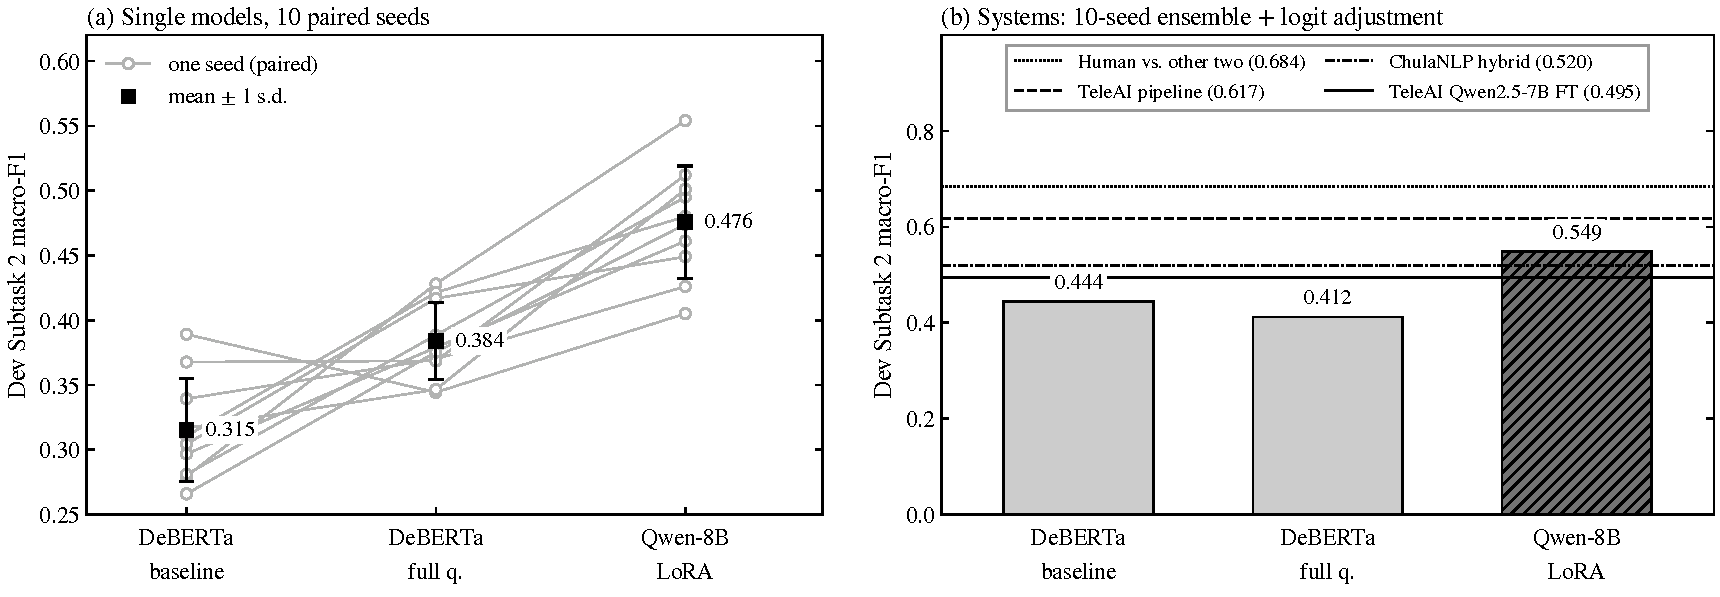
\includegraphics[width=0.96\textwidth]{figures/qwen_vs_deberta.pdf}
  \begin{itemize}\small
    \item Same rows, input and selection rule. Qwen3-8B-Base + LoRA replaces DeBERTa. Single model 0.384 $\rightarrow$ \hl{0.476}, \hl{10/10 seeds up}.
    \item Systems in (b) are means over 10 nested-CV splits. Qwen passes TeleAI's fine-tuned 7B (0.495) and ChulaNLP's hybrid (0.520).
  \end{itemize}
\end{frame}

% 13
\begin{frame}{The gain is broad, not one boundary}
  \begin{columns}[c]
    \begin{column}{0.6\textwidth}
      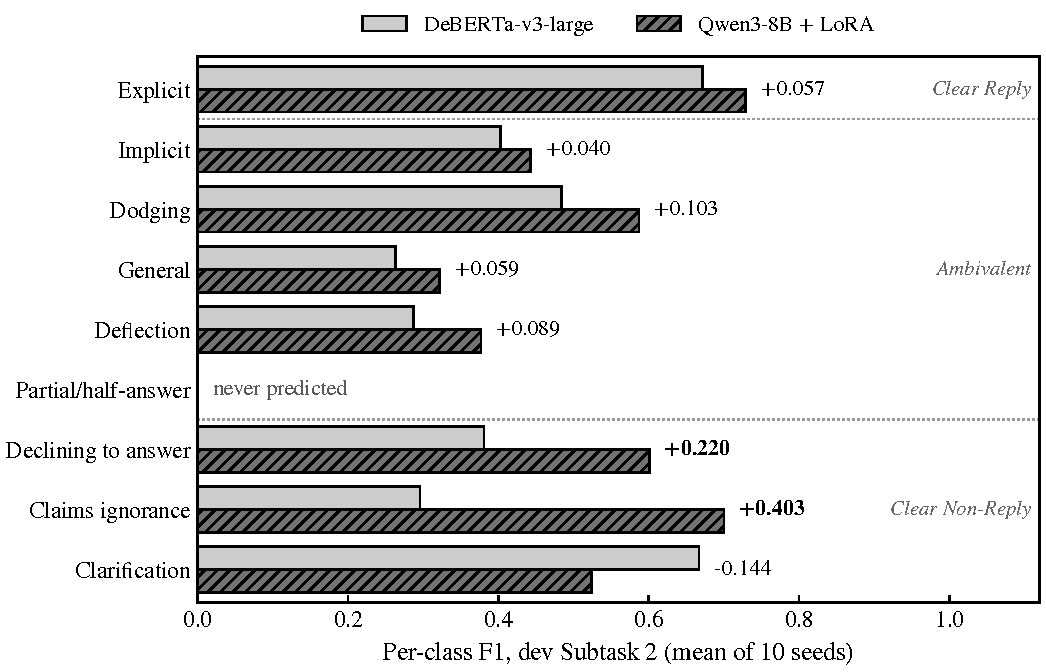
\includegraphics[width=\linewidth]{figures/per_class_gain.pdf}
    \end{column}
    \begin{column}{0.38\textwidth}
      \small
      \begin{itemize}
        \item Seven of nine classes improve, most in Claims ignorance (\hl{+0.403}) and Declining (+0.220).
        \item Clarification has only 4 dev items, so its F1 swings widely ($-0.144$ here).
        \item We predicted gains on the Explicit/Implicit boundary. That prediction was refuted.
      \end{itemize}
    \end{column}
  \end{columns}
\end{frame}

% 14
\begin{frame}{The model ranks better than it decides}
  \centering
  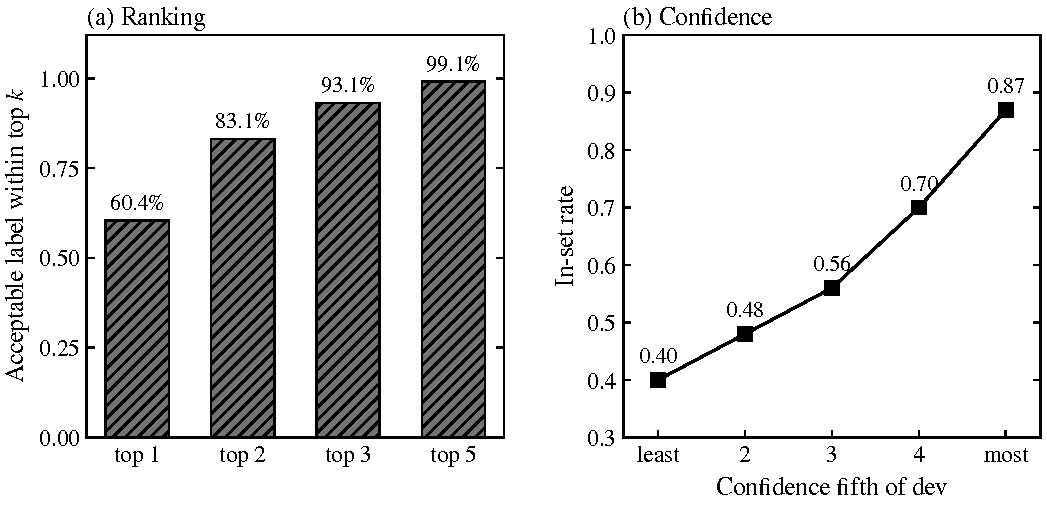
\includegraphics[height=0.6\textheight]{figures/ranking_vs_decision.pdf}
  \begin{itemize}\small
    \item Qwen3-8B (3 epochs, seeds 0--2): an acceptable label is first for 60.4\% of items but in the top 3 for \hl{93.1\%}.
    \item Confidence tracks correctness (in-set rate 0.40 $\rightarrow$ 0.87), so we can route only the uncertain items to a stronger chooser.
  \end{itemize}
\end{frame}

% 15
\begin{frame}{The final system: a confidence-routed cascade}
  \centering
  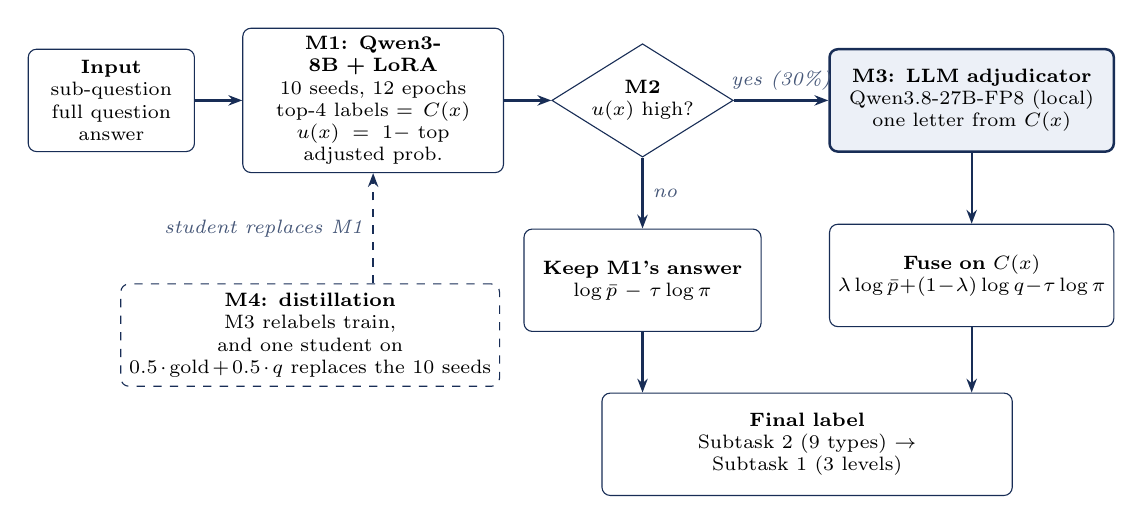
\begin{tikzpicture}[
      font=\scriptsize,
      box/.style={draw=navy, rounded corners=3pt, align=center, fill=white, minimum height=13mm, inner sep=3pt},
      main/.style={box, fill=soft, line width=0.9pt},
      arr/.style={-{Stealth[length=5pt]}, navy, thick},
      lab/.style={font=\scriptsize\itshape, text=navy!80}]
    \node[box, text width=19mm] (in) {\textbf{Input}\\sub-question\\full question\\answer};
    \node[box, text width=31mm, right=6mm of in] (m1) {\textbf{M1: Qwen3-8B + LoRA}\\10 seeds, 12 epochs\\top-4 labels $=C(x)$\\$u(x)=1-$ top adjusted prob.};
    \node[draw=navy, diamond, aspect=1.6, inner sep=1pt, align=center, right=6mm of m1] (m2) {\textbf{M2}\\$u(x)$ high?};
    \node[main, text width=34mm, right=12mm of m2] (m3) {\textbf{M3: LLM adjudicator}\\Qwen3.8-27B-FP8 (local)\\one letter from $C(x)$};
    \node[box, text width=28mm, below=9mm of m2] (keep) {\textbf{Keep M1's answer}\\$\log\bar p - \tau\log\pi$};
    \node[box, text width=34mm, below=9mm of m3] (fuse) {\textbf{Fuse on $C(x)$}\\$\lambda\log\bar p+(1-\lambda)\log q-\tau\log\pi$};
    \node[box, text width=50mm, below=8mm of $(keep.south)!0.5!(fuse.south)$] (out) {\textbf{Final label}\\Subtask 2 (9 types) $\rightarrow$ Subtask 1 (3 levels)};
    \node[box, dashed, text width=46mm, below=14mm of m1, xshift=-8mm] (m4) {\textbf{M4: distillation}\\M3 relabels train, and one student on\\$0.5\cdot\text{gold}+0.5\cdot q$ replaces the 10 seeds};
    \draw[arr] (in) -- (m1);
    \draw[arr] (m1) -- (m2);
    \draw[arr] (m2) -- node[lab, above] {yes (30\%)} (m3);
    \draw[arr] (m2) -- node[lab, right] {no} (keep);
    \draw[arr] (m3) -- (fuse);
    \draw[arr] (keep) -- (keep |- out.north);
    \draw[arr] (fuse) -- (fuse |- out.north);
    \draw[arr, dashed] (m1.south |- m4.north) -- node[lab, left] {student replaces M1} (m1.south);
  \end{tikzpicture}
  \vspace{4pt}
  \begin{itemize}\small
    \item Only the least confident items reach the LLM. $\delta=0.3$, with the threshold set on the train slice, gives \hl{0.36 calls per item} on dev. Confident items keep M1's answer.
    \item Everything is chosen on train or by nested cross-validation. Dev only reports.
  \end{itemize}
\end{frame}

% 16
\begin{frame}{The four modules in brief}
  \begin{columns}[T]
    \begin{column}{0.48\textwidth}
      \modcard{M1 \quad Candidate generator}
        {Qwen ranks well but decides poorly (gold in its top 3 for 93\% of items).}
        {Qwen3-8B + LoRA, 12 epochs, 10 seeds, ensemble + logit adjustment. Outputs the top-4 set $C(x)$ and an uncertainty $u(x)$.}
        {\hl{0.598} S2 / 0.743 S1 alone, with no LLM call.}
      \modcard{M3 \quad LLM adjudicator}
        {a larger model knows more, but calling it on every item is costly.}
        {a local 27B LLM picks one letter from $C(x)$. Its distribution $q$ is fused with M1's.}
        {\hl{0.669} S2 / 0.798 S1, +0.067 over M1 [+0.009, +0.124]. 33 items fixed, 9 broken.}
    \end{column}
    \begin{column}{0.48\textwidth}
      \modcard{M2 \quad Uncertainty router}
        {confidence tracks correctness (in-set rate 0.40 $\rightarrow$ 0.87 across confidence fifths).}
        {send only the $\delta$ least-confident items to M3. Threshold set on the train slice.}
        {$\delta=0.3$ gives \hl{0.36 calls/item}. Sending every item is worse (0.609 vs 0.660).}
      \modcard{M4 \quad Distillation}
        {the 10 seeds are 93\% of the compute at the accuracy point.}
        {M3 relabels train. One student learns from $0.5\cdot\text{gold}+0.5\cdot q$.}
        {student + M3: \hl{0.608} S2 at 0.111 GPU-s per item, 4.7$\times$ cheaper than M1 alone.}
    \end{column}
  \end{columns}
\end{frame}

% 17
\begin{frame}{M1 + M2 + M3: the cascade on dev}
  \begin{columns}[T]
    \begin{column}{0.56\textwidth}
      \small
      \begin{tabular}{@{}lcccc@{}}
        \toprule
        $\delta$ & calls & S2 & S2 (10 splits) & S1 \\
        \midrule
        0 (M1) & 0 & 0.598 & 0.601 & 0.743 \\
        0.1 & 0.11 & 0.597 & 0.602 & 0.762 \\
        0.2 & 0.23 & 0.635 & 0.640 & 0.775 \\
        \textbf{0.3} & \textbf{0.36} & \textbf{0.669} & \textbf{0.660} & \textbf{0.798} \\
        0.5 & 0.65 & 0.628 & 0.628 & 0.800 \\
        1 & 1.00 & 0.636 & 0.609 & 0.798 \\
        \bottomrule
      \end{tabular}
      \vspace{4pt}

      \footnotesize $\delta$ = target share deferred (threshold set on the train slice, realised calls in column 2).
    \end{column}
    \begin{column}{0.42\textwidth}
      \small
      \begin{itemize}
        \item M1 alone (12 epochs, 10 seeds): \hl{0.598} with no LLM call.
        \item At $\delta=0.3$: \hl{+0.067} [+0.009, +0.124]. 33 items fixed, 9 broken.
        \item Deferring every item is worse (0.609). The router matters.
        \item Screened on train: no examples, local 27B over DeepSeek V4 Flash and Gemma 4 31B. API spend \$0.26.
      \end{itemize}
    \end{column}
  \end{columns}
\end{frame}

% 18
\begin{frame}{Cost: one distilled student replaces ten seeds}
  \begin{columns}[c]
    \begin{column}{0.5\textwidth}
      \centering
      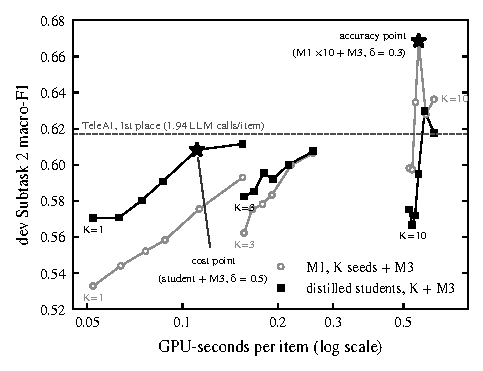
\includegraphics[width=0.8\linewidth]{figures/E18_frontier.pdf}
      \par\vspace{2pt}\raggedright
      \scriptsize
      \textbf{Measured} on one RTX PRO 6000: an M1 seed costs 0.0522 GPU-s per item, an M3 call 0.103.\\[2pt]
      \renewcommand{\arraystretch}{1.1}
      \begin{tabular}{@{}l@{\ }l@{}}
        M1 $\times$ 10: & $10\times0.0522 = \mathbf{0.522}$ \\
        Accuracy point: & $0.522 + 0.357\times0.103 = \mathbf{0.558}$ (seeds = 93\%) \\
        Cost point: & $0.0522 + 0.574\times0.103 = \mathbf{0.111}$ \\
        & $0.522/0.111 = $ \hl{4.7$\times$} cheaper than M1 $\times$ 10 \\
      \end{tabular}
    \end{column}
    \begin{column}{0.48\textwidth}
      \begin{block}{The student's target (M4)}
        \footnotesize
        \[ t(c) = 0.5\cdot\mathbb{1}[c=\text{gold}] + 0.5\cdot q(c) \]
        \vspace{-4pt}
        \begin{itemize}
          \item $q$: M3's softmax over the 4 candidate letters, 0 outside $C(x)$.
          \item \textbf{Why gold:} anchors the student to the annotators where M3 is wrong.
          \item \textbf{Why $q$:} says \emph{which} other labels are plausible, knowledge a one-hot label throws away.
          \item The 0.5 mix was fixed in advance, not tuned.
        \end{itemize}
      \end{block}
      \scriptsize
      \begin{itemize}
        \item Student alone: 0.573 per model (+0.048, 9/10 seeds up).
        \item Student + M3 ($\delta=0.5$): \hl{0.608} S2 / 0.790 S1 at \hl{0.111 GPU-s}, above M1 $\times$ 10 alone (0.598 at 0.522).
      \end{itemize}
    \end{column}
  \end{columns}
\end{frame}

% 19
\begin{frame}{Final results (dev, 308 items)}
  \centering
  \footnotesize
  \begin{tabular}{@{}lcccc@{}}
    \toprule
    System & Subtask 2 & Subtask 1 & LLM calls & GPU-s \\
           &           &           & per item  & per item \\
    \midrule
    DeBERTa-v3-large, 10-seed system & 0.405 & 0.648 & 0 & -- \\
    Qwen3-8B + LoRA, 3 epochs, 10 seeds (mid-evaluation) & 0.543 & 0.746 & 0 & -- \\
    M1: Qwen3-8B, 12 epochs, 10 seeds & 0.598 & 0.743 & 0 & 0.522 \\
    \textbf{Accuracy point: M1 $\times$ 10 + M3, $\delta=0.3$} & \textbf{0.669} & \textbf{0.798} & 0.36 & 0.558 \\
    \textbf{Cost point: student + M3, $\delta=0.5$} & \textbf{0.608} & \textbf{0.790} & 0.57 & 0.111 \\
    \midrule
    TeleAI, 1st place (DeepSeek-V3, three stages) & 0.617 & 0.812 & 1.94 & -- \\
    One human annotator vs.\ the other two & 0.684 & -- & -- & -- \\
    \bottomrule
  \end{tabular}
  \vspace{8pt}
  \begin{itemize}\small
    \item The accuracy point is above the winning system on Subtask 2 with \hl{a fifth of its LLM calls}, and 1 output token per call.
    \item The cost point still beats M1 $\times$ 10 alone while costing \hl{4.7$\times$ less} compute.
  \end{itemize}
\end{frame}

% 20
\begin{frame}{Conclusions, limitations and what comes next}
  \begin{columns}[T]
    \begin{column}{0.48\textwidth}
      \begin{block}{What we learned}
        \footnotesize
        \begin{itemize}
          \item Knowledge, not structure: changing only the backbone gained more (+0.092 per model) than all encoder-side changes combined (+0.069).
          \item A 27B LLM, deciding only uncertain items among four candidates, beats the winning multi-call pipeline on Subtask 2 (not yet on Subtask 1).
          \item Distillation turns the cascade's accuracy into a cheap single model.
        \end{itemize}
      \end{block}
      \begin{block}{Limitations}
        \footnotesize
        \begin{itemize}
          \item Dev has only 308 items. The M3 gain interval is wide, and seed-subset averages suggest +0.02 to +0.04.
          \item Partial/half-answer (F1 0.40) and General (0.51) remain the weakest classes.
        \end{itemize}
      \end{block}
    \end{column}
    \begin{column}{0.48\textwidth}
      \begin{block}{What comes next}
        \footnotesize
        \begin{itemize}
          \item \textbf{Adaptive candidate sets}: let $|C(x)|$ grow on hard items instead of a fixed top 4.
          \item \textbf{A sharper teacher}: tune the gold/$q$ mix and a temperature on $q$, and distil again.
          \item \textbf{Close the Subtask 1 gap} (0.798 vs 0.812) with fusion that respects the taxonomy.
          \item \textbf{Weak classes}: targeted examples for Partial/half-answer and General.
        \end{itemize}
      \end{block}
      \vspace{2pt}
      \centering\footnotesize\textcolor{navy}{\textbf{A small model that knows when to ask a bigger one.}}
    \end{column}
  \end{columns}
\end{frame}

\end{document}
